\subsection{Language Models} \label{language_models}
Since the Entity Typing task deals with textual features, we need to introduce some basic concepts regarding text representation. Over the years, a lot of approaches have been proposed to transform the text into a machine-readable format, reaching more and more effectiveness in several downstream Natural Language Processing (NLP) tasks. A wide variety of language models is available, providing different ways to represent textual information in a vectorial space. Choosing the right language model is crucial when facing NLP problems and could be decisive to achieve quality results: if we start from a low-quality text representation, we cannot expect high-quality results for any following task~\cite{babic2020survey}. 

Before proceeding with the overview, it is good to provide a general definition of language model: \textit{a language model is a statistical model which represents probability distributions over sequences of words}. Given a sequence of words \\$W=w{1},...,w_{n}$, a language model is able to compute $P(W)$ or \\$P(w_{n+1} | w_{1},...,w_{n})$. 

\subsubsection{Overview}
The first approaches were based on the frequencies of the words in a corpus. The classic example is the Bag Of Word (BOW) model. Introduced by Zellig Harris in 1954~\cite{harris1954distributional}, it has become the starting point of many future works. This approach has lots of limitations, especially the sparsity of its high-dimensionality vectors. To overcome these limits, other valid solutions have been proposed through the years under the name of Word Embeddings. The common goal of these newer approaches is to map the words of a vocabulary from a high-dimensionality space into a real vector space with low-dimensionality. Word Embeddings rely on the distributional hypothesis for which similar words tend to appear in similar contexts. These models can be grouped into two main categories: count-based models and predictive models.

One of the most popular count-based approaches is GloVe~\cite{pennington2014glove}. It captures the statistics of a corpus by computing word-word co-occurrences, then for each pair of words it optimizes an objective that relates co-occurrences to contexts. 

Moving on to predictive models, we can find the famous Skip-Gram (SG) and Continuous Bag Of Words (CBOW) methods. Best known as Word2Vec, they are based on neural networks. For both models, the embedding vectors correspond to the learned weights of the hidden layer of the network. The aspect that distinguishes the two approaches is that while CBOW is trained to predict the central word of a sliding window given the context words, SG is trained to predict context words given the central word. With both methodologies, it is possible to learn high-quality word vectors maintaining low-dimensionality, where vector similarity can be measured using the cosine similarity. The more two words have similar meanings, the closer they will be in the vector space.

In 2017 the advent of transformers had an important impact in the NLP research area. The publication~\cite{vaswani2017attention} introduced this new neural architecture based on encoders and decoders. Transformers rely on a sequence-to-sequence architecture and were originally used for machine translation. Differently from Recurrent Neural Networks (RNN), which operate on sequences and are intrinsically sequential, transformers operate on sets in a parallel way. Instead of using a single compressed encoding coming from the last encoder like in RNN, in transformers the decoders can access the information of each input element. The core of these models is the Self-Attention mechanism that is applied to the input tokens of each transformer encoder/decoder. This operation makes the model able to capture deeper contextual information and dependencies, thus providing a much better representation than the previous approaches. Since the attention operation works on sets and not on sequences, the model can be constrained by adding positional encodings to deal with text sequences. Transformers architecture inspired future works like BERT~\cite{devlin-etal-2019-bert} and GPT~\cite{gpt}, which gained more and more popularity until nowadays. They both exploit a mechanism based on Self-Attention, but while the first is composed of a stack of transformer encoders, the latter is constituted by a stack of transformer decoders.

\subsubsection{BERT}
Inspired from transformers, Devlin et al. presented BERT (Bidirectional Encoder Representations from Transformers) in 2019~\cite{devlin-etal-2019-bert}. Unlike the original transformer architecture, it does not use any decoder. The fact that it uses a stack of 12 bidirectional transformer encoders makes BERT able to exploit both the left and right context of each word. Moreover, thanks to the attention mechanism inherited from transformers, this architecture can be used to generate very powerful language models with dense neural representation.

Before feeding the model, the input text is transformed into a sequence in the form of WordPiece embeddings~\cite{wordpiece} with a vocabulary counting 30,000 tokens. Using this representation, each word is decomposed into subwords, thus allowing to improve the handling of rare words. The format of an input sequence can contain special tokens like \verb|[CLS]| and \verb|[SEP]|. The first one is the \textit{classification token} and its final hidden state can be used as the aggregate sequence representation for classification tasks. The latter stands for \textit{separator token} and can be used when we need to differentiate the sentences which constitute the input. 

BERT earned most of its popularity thanks to the fact that it can be used in a wide variety of NLP downstream tasks without big efforts. Indeed, it comes as a model pre-trained on a large amount of data and provides a generic language representation that can be fine-tuned to face any problem (e.g., Question Answering, classification, NER, etc.). A sketch of the training procedure is shown in Figure~\ref{fig:bert_training}. The pre-training procedure is performed using two strategies:
\begin{enumerate}
    \item \textbf{Masked Language Model:} for each input sequence, the 15\% of tokens are replaced by the \verb|[MASK]| token. Then, the model is trained to predict the original values of the masked tokens by exploiting the left and right context.
    % In this way, BERT will learn a token/embedding matrix.
    \item \textbf{Next Sentence Prediction (NSP):} each input sequence is split into two parts separated by the \verb|[SEP]| token. Then, the 50\% of the sequences get modified by replacing the second part using a random one from another sequence. Finally, the model is trained to distinguish positive and negative sequences.
    % In this way, BERT will learn full sentence embeddings.
\end{enumerate}

\begin{figure}[H]
    \centering
    \centerline{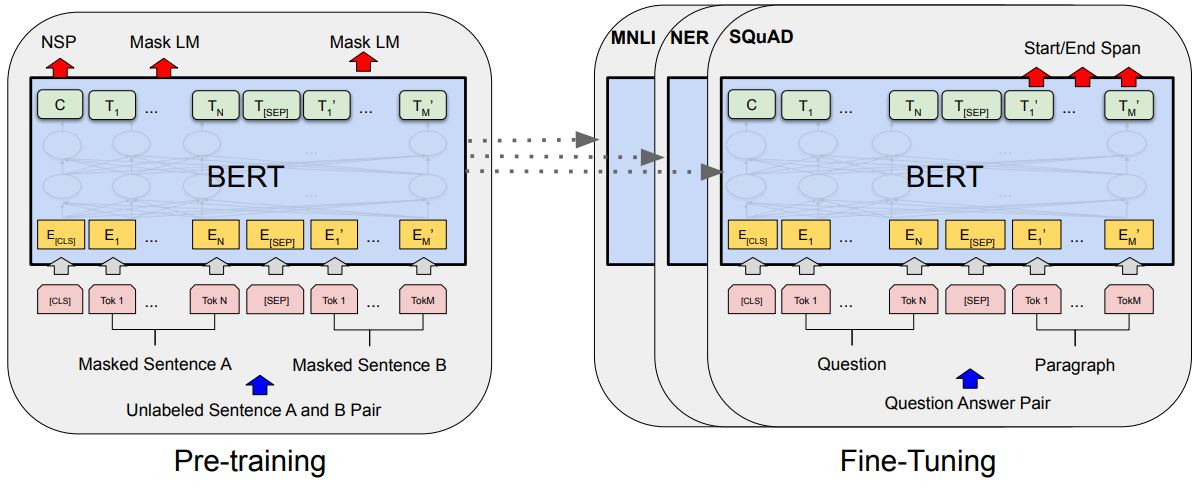
\includegraphics[scale=.5]{figures/bert_training.JPG}}
    \caption{BERT's pre-training and fine-tuning. (Source:~\cite{devlin-etal-2019-bert})}
    \label{fig:bert_training}
\end{figure}

Until now, we only talked about the strengths of BERT. However, the high quality of the text representation is achieved at the expense of high resources usage. BERT's model comes originally in two versions: BERT base (110M parameters) and BERT large (340M parameters). These model sizes require high memory capabilities and make the training procedure not accessible to everyone. For this reason, different new versions have been proposed over the last few years and several examples can be found at HuggingFace\footnote{https://huggingface.co/models}. Among these versions, we can find BERT-based models which are lighter than the original (e.g., DistilBERT, RoBERTa, etc.) and models fine-tuned for specific tasks or different languages.



\subsubsection{DistilBERT}
As suggested by the name, DistilBERT is a distilled version of BERT~\cite{distilbert}. With 40\% fewer parameters, it is 35\% faster at inference time and it is effective at 97\% with respect to the performance of the original version of BERT. Thanks to its lighter architecture composed of only 6 transformer encoders, it can be fine-tuned in a more reasonable time. DistilBERT model is pre-trained using knowledge distillation. This procedure is a compression technique in which a smaller \textit{student} model (i.e., DistilBERT) is trained to emulate a larger \textit{teacher} model (i.e., BERT).

\subsubsection{Adapters}
The fine-tuning of a model requires less time than training it from scratch. However, even this procedure can be quite expensive, especially when dealing with very large models. An alternative solution to adapt a BERT-based model to a new task can be found in the \textit{adapters}~\cite{pfeiffer-etal-2020-mad,pfeiffer2021adapterfusion}. The key concept behind the adapters is to introduce a small set of learnable parameters for each transformer layer. In the case of BERT and its variants, these parameters are added to each transformer encoder. The training is then performed by freezing all the weights of the pre-trained language model and updating only the parameters introduced by the adapters. As shown in Figure~\ref{fig:adapters}, the new parameters can be added following two strategies:
\begin{itemize}
    \item \textbf{Pfeiffer:} an adapter is added after each transformer encoder (Figure~\ref{fig:adapters_pfeiffer})
    \item \textbf{Houlsby:} two adapters are added for each transformer encoder, one after the attention layer and one after the feedforward layer (Figure~\ref{fig:adapters_houlsby})
\end{itemize}

\begin{figure}[H]
     \centering
     \begin{subfigure}[b]{0.3\textwidth}
         \centering
         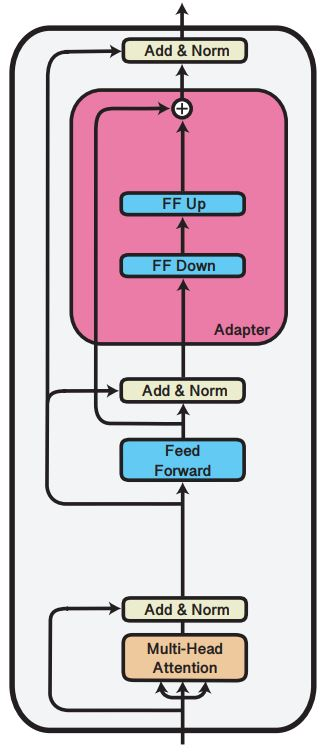
\includegraphics[width=\textwidth]{figures/adapters_pfeiffer.JPG}
         \caption{Pfeiffer strategy}
         \label{fig:adapters_pfeiffer}
     \end{subfigure}
     \hspace{40px}
     \begin{subfigure}[b]{0.302\textwidth}
         \centering
         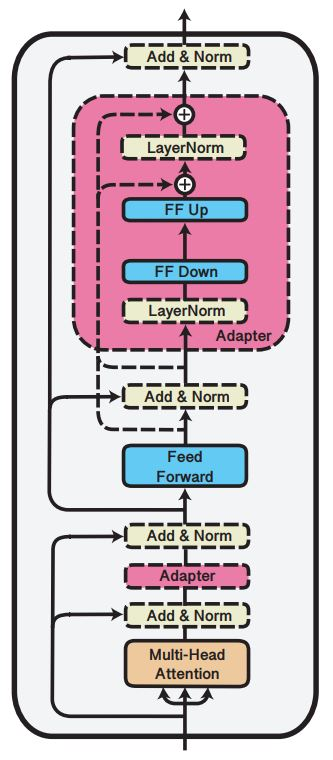
\includegraphics[width=\textwidth]{figures/adapters_houlsby.JPG}
         \caption{Houlsby strategy}
         \label{fig:adapters_houlsby}
     \end{subfigure}
    \caption{Adapters architectures. (Source:~\cite{pfeiffer2021adapterfusion})}
    \label{fig:adapters}
\end{figure}

The modifications introduced by both the architectures can be seen as the addition of auto-encoders to the model. The dimensionality of the input is reduced (with respect to a customizable reduction factor) through a first feedforward layer (FF-DOWN in Figure~\ref{fig:adapters}) and then expanded to its original size through another feedforward layer (FF-UP in Figure~\ref{fig:adapters}). In this way, a pre-trained model can adapt to new tasks without requiring any fine-tuning of the original weights. In addition, Pfeiffer et al. show in~\cite{pfeiffer2021adapterfusion} that their approach outperforms traditional strategies such as full fine-tuning as well as multitask learning.